%----------------------------------------------------------------------------------------
%	SECTION 1.5
%----------------------------------------------------------------------------------------

\section{Continuous Functions.}

\begin{definition}
    Let $X$ and  $Y$ be topological spaces. We say that a mapping $f:X
    \rightarrow Y$ is  \textbf{continuous} if for each open set $V$ in  $Y$,
    $f^{-1}(V)$ is open in $X$.
\end{definition}

Now if $f:X \rightarrow Y$ is continuous, the for every open set  $V$ of  $Y$,
$f^{-1}(V)$ is open in  $X$. Now suppose that  $\Bc$ is a basis of  $Y$, then
$V=\bingcup{B_{\alpha}}$, hence
$f^{-1}(\bingcup{B_{\alpha}})=\bingcup{f^{-1}{B_{\alpha}}}$, which is open in
$X$, thus  $B_{\alpha}$ must also be open in  $X$. 

Similarly, if $\Sc$ is a subbasis of  $Y$, then for any basis element  $B$ of
$Y$,  $B=\bigcap_{i=1}^{n}{S_i}$, which then implies that
$f^{-1}(B)=\bigcap_{i=1}^{n}{f^{-1}(S_i)}$, thus  $S_i$ is also open in  $X$ for
 $1 \leq i \leq n$.

\begin{example}
    \begin{enumerate}[label=(\arabic*)]
        \item Let $f:\R \rightarrow \R$ be a continuous realvalued function.
            THen for each open interval  $I \subseteq \R$,  $f^{-1}(I)$ is an
            open interval in  $\R$, so take  $x_0 \in \R$ and $\epsilon>0$, and
            let $I=(f(x_0)-\epsilon,f(x_0)+\epsilon)$, then since $ x_0 \in
            f^{-1}(I)$, there is a basis $(a,b) \subseteq f^{-1}(I)$ about
            $x_0$. Then take  $\delta=\min\{x_0-a,x_0-b\}$, then $x \in (a,b)$
            whenever $0<|x-x_0|<\delta$, and we get that $f(x) \in I$, that is,
            $|f(x)-f(x_0)|<\epsilon$. This is the definition of continuity
            defined in the real analysis. We can prove that the converse holds
            also.

            If $f:\R \rightarrow \R$ is continuous at a point $x_0$, then for
            every $\epsilon>0$, there is a  $\delta>0$ such that
            $|f(x)-f(x_0)|<\epsilon$ whenever $0<|x-x_0|<\delta$. Then we notice
            that $x$ and  $ x_0$ are distinct, furthermore, $x_0-\delta<x
            <x_0+\delta$, hence $x \in (x_0-\delta,x_0+\delta)$ implies that
            $f(x) \in (f(x_0)-\epsilon,f(x_0)+\epsilon)$. Letting
            $V_{\delta}(x_0)=(x_0-\delta,x_0+\delta) $ and
            $V_{\epsilon}(f(x_0))=(f(x_0)-\epsilon,f(x_0)+\epsilon)$, we have
            that whenever  $x \in V_{\delta}(x_0)$, then $f(x) \in
            V_{\epsilon}(f(x_0)) \subseteq f^{-1}(V_{\delta}(x_0))$. And so the
            topological definition of continuity is equivialent to the real
            analytic definition of continuity.

        \item Let $f:\R \rightarrow \R_l$ be defined such that  $f(x)=x$ for all
            $x \in \R$. Take  $[a,b) \subseteq \R_l$, we have that
            $f^{-1}([a,b))=[a,b)$, which is not open in  $\R$  (under the
            standard topology), hence $f$ is not continuous. However, the map
            $g:\R_l \rightarrow \R$ defined the same way is continuous since
            $g^{-1}((a,b))$ is open in  $\R_l$.
    \end{enumerate}
\end{example} 

\begin{theorem}\label{1.7.1}
    Let $X$ and  $Y$ be topological spaces, and let  $f:X \rightarrow Y$ be a mapping of  $X$ into
    $Y$. Then the following are equivalent:
        \begin{enumerate}[label=(\arabic*)]
            \item $f$ is continuous.

            \item For every $A \subseteq X$,  $f(\cl{A}) \subseteq \cl{f(A)}$.

            \item For every closed set $B \subseteq Y$,  $f^{-1}(B)$ is closed in $X$.

            \item For each  $x \in X$ and each neighborhood  $V$ of  $f(x)$, there us a neighborhood
                $U$ of  $x$ such that  $f(U) \subseteq V$.
        \end{enumerate}
\end{theorem}
\begin{proof}
    Let $f$ be continuous and let  $A \subseteq X$. Consider the neighborhood  $V$ of  $f(x)$, then
    $f^{-1}(V)$ is open in $X$, and intersects  $A$ at a point  $y$. Then  $V \cap f(A)=f(y)$, thus 
    $f(x) \in \cl{f(A)}$.

    Now let $B$ be closed in  $Y$, and let  $A=f^{-1}(B)$. THen we have that $f(A)=f(f^{-1(B)})
    \subseteq B$, thus $x \in \cl{A}$.

    Now let $V$ be open in $Y$, so that  $B=\com{Y}{V}$ is closed in $Y$, and
    $f^{-1}(B)=\com{f^{-1}(Y)}{f^{-1}(V)}=\com{X}{f^-1}(V)$ which is closed in $X$, hence
    $f^{-1}(V)$ is open in $X$.

    Now let  $x \in X$, and let  $V$ be a neighborhood of  $f(x)$. Then $U=f^{-1}(V)$ is a
    neighborhood of $x$ for which  $f(U) \subseteq V$. Finally let $V$ be open in  $Y$, and let $x
    \in f^{-1}(V)$, then $f(x) \in V$, so  there is a neighborhood $U_x$ of  $x$ for which  $f(U_x) \subseteq V$,
    then $U_x \subseteq f^{-1}(V)$, then $f^{-1}(V)$ is a union of open sets, and hence open in $X$.
\end{proof}

\begin{definition}
    Let $X$ and  $Y$ be topological spaces, and  $f:X \rightarrow Y$ be a $1-1$ mapping of  $X$ onto
    $Y$. We call  $f$ a \textbf{homeomorphism} if both $f$ and  $f^{-1}$ are continuous.		
\end{definition}

\begin{lemma}\label{1.7.2} 
    Let $X$ and  $Y$ be topological spaces and let $f:X \rightarrow Y$ be a homeomorphism. Then
    $f(U)$ is open if and only if $U$ is open.
\end{lemma}
\begin{proof}
    We have that both $f:X \rightarrow Y$ and  $f^{-1}:Y \rightarrow X$ are continuous $1-1$ of $X$
    and  $Y$ onto each other  (respectively). Now let $U$ be open in  $X$, then $U=f^{-1}(V)$, for 
    some set  $V$ open in $Y$. Notice then, that $f(U)=f(f^{-1}(V))=V$, thus $f(U)$ is open in $Y$. 
    Conversely, let $V=f(U)$ be open in $Y$ for some open set  $U$ in  $X$, then  $U=f^{-1}(V)$, so
    by definition of continuity, $U$  is open in $X$.
\end{proof}

\begin{definition}
    Let $X$ and  $Y$ be topological spaces and let  $f:X \rightarrow Y$ be a contiuous  $1-1$ maping
    of  $X$ into  $Y$, and consider  $f(X)$ as a subspace of $Y$. We call  $f:X \rightarrow f(X)$ a
    \textbf{topological imbedding} if $f$ is a homeomorphism of $X$ onto  $f(X)$.
\end{definition}

\begin{example}
    \begin{enumerate}[label=(\arabic*)]
        \item The map $f:\R \rightarrow \R$ defined by  $f(x)=3x+1$ is a homeomorphism whose inverse
            is $f^{-1}(y)-\frac{1}{3}(y-3)$, both $f$ and  $f^{-1}$ are contiuous.

        \item The map $f:(-1,1) \rightarrow \R$ defined by $f(x)=\frac{x^2}{1-x^2}$ has as its
            inverse the map $f:\R \rightarrow (-1,1)$ defined by
            $f^{-1}(y)=\frac{2y}{1+\sqrt{1+4y^2}}$. Both $f$ and  $f^{-1}$ are contiuous, so $f$ is
            a homeomorphism.

        \item Teh map  $g:\R_l \rightarrow \R$ defined by  $g(x)=x$ is not a homeomorphism, despite
            being contiuous, as $g^{-1}(1)$ is undefined.

        \item Let $S^1$ be the unit circle in $\R$, which is a subspace of $\R$, and define
            $f:[0,1) \rightarrow S^1$ by $f(t)=(\cos(t),\sin(t))$. Clearly $f$ is  $1-1$ onto
            $S^1$, and contiuous, however  $f^{-1}$ is not contiuous as $f([0,\frac{1}{4}))$ is not
            open in $S^1$ as  $f(0)$ is in no open set of $\R^2$ such that  $U \cap S^1=f([0,1))$.

        \item Consider the mappings $g:[0,1) \rightarrow \R^2$ by $f(t)=(\cos(2t\pi),\sin(2t\pi)))$.
            Now $g$ is  $1-1$ and continuous, and we have that  $g([0,1)) \subseteq S^1$, however
            since $g$ is not a homeomorphism,  $g$ fails to be a topological embedding.
    \end{enumerate}
\end{example} 

\begin{theorem}[Constructions for continuous functions.]\label{1.7.3}
    Let $X$ and  $Y$ be topological spaces, then:
        \begin{enumerate}[label=(\arabic*)]
            \item (Constant construction) If $f:X \rightarrow Y$ maps  $x \rightarrow y_0$ for all
                $x \in X$, then  $f$ is continuous.

            \item  (Inclusion) If $A \subseteq X$ is a subspace, then the inclusion mapping  $\iota:A
                \rightarrow Y$ is continuous.

            \item (Construction by composition) If $f:X \rightarrow Y$ and  $g:Y \rightarrow Z$ are
                continuous, then  $f \circ g: X \rightarrow Z$ is also continuous.

            \item  (Domain restriction) If  $f:X \rightarrow Y$ is continuous and  $A \subseteq X$,
                then  $f:A \rightarrow Y$ is continuous.

            \item  (Range restriction) if $f:X \rightarrow Y$, and  $Z \subseteq Y$ such that  $f(X)
                \subseteq Y$, then $f:X \rightarrow Z$ is continuous.

            \item  (Range exapnsion) If $f:X \rightarrow Y$ is continuous, and  $Y \subseteq Z$ is a
                subspace of  $Z$, then  $f:X \rightarrow Z$ is continuous.

            \item  (Local Formulation) The map $f:X \rightarrow Y$ is continuous if  $X$ can be
                written as the union of open sets  $U_{\alpha}$ such that $f:U_{\alpha} \rightarrow
                Y$ is continuous for all $\alpha$.
        \end{enumerate}
\end{theorem}
\begin{proof}
    \begin{enumerate}[label=(\arabic*)]
        \item Let $f (x)=y_0$ for all $x \in X$, and let  $V$ be open in  $Y$, then  $f^{-1}(V)=X$
            or $\emptyset$ depending on if $ y_0 \in V$ or noy. In either case, $f^{-1}(V)$ is open.

        \item If $U$ us open in  $X$, then  $f^{-1}(U)=U \cap A$ which is open in the subspace
            topology of $X$.

        \item If $U$ is open in  $Z$,  $g^{-1}(U)$ is open in $Y$, hence  $f^{-1}g^{-1}(U)$ is
            open in $X$.

        \item Notice that  $f_A=\iota \circ f=f:A \rightarrow Y$ which is continuous by $(2)$
            and $(3)$.

        \item Let $f:A \rightarrow Y$ be continuous and let  $f(X) \subseteq Z \subseteq Y$. Let $B$
            be open in  $Z$, so  $B=Z \cap U$ for some  $U$ open in  $Y$. Now by hypothesis, we have
            that $f^{-1}(U) \subseteq f^{-1}(B)$, hence $f^{-1}(B)$ is open in $X$, thus  $f:X
            \rightarrow Z$ is continuous.

        \item Let  $f$ be as in  $(5)$, and let $Y \subseteq Z$ be a subspace of  $Z$. Then the
            mapping  $h:X \rightarrow Z$ defined by $h=\iota \circ f$ is continuous.

        \item Let  $X=\bingcup{U_{\alpha}}$ where $U_{\alpha}$ is open in $X$, and $f:U_{\alpha}
            \rightarrow Y$ is continuous for all  $\alpha$. LEt $V$ be open in  $Y$, then
            $f^{-1}(V) \cap U_{\alpha}=f^{-1}_U{\alpha}(V)$, and since $f$ is continuous on
            $U_{\alpha}$, then $f^{-1}(V)=\bigcup{f^{-1}_{U_{\alpha}}(V)}$ is open in $X$.
    \end{enumerate}
\end{proof}

\begin{theorem}[The pasting lemma]\label{1.7.4}
    Let $X=A \cap B$ with  $A$ and  $B$ closed in  $X$, and let  $f:A \rightarrow Y$ and  $g:B
    \rightarrow Y$ be continuous. If  $f(x)=g(x)$ for all $x \in A \cap B$, then we can
    construct a mapping  $h:X \rightarrow Y$ defined by  $h(x)=
        \begin{cases}
            f(x) \text{, } & x \in A \\
            g(x) \text{, } & x \in B
        \end{cases}$
    . Then $h$ is continuous.
\end{theorem}
\begin{proof} 
    Let $C$ be closed in  $Y$, then  $h^{-1}(C)=f^{-1}(C) \cup g^{-1}(C)$. Since $f$ and  $g$ are
    continuous, then  $f^{-1}(C)$ and $g^{-1}(C)$ are closed in $A$ and  $B$, respectively. Thus
    $h^{-1}(C)$ is closed in $X$.
\end{proof}

\begin{example}
        Define $h:\R \rightarrow \R$ by $h(x)=
            \begin{cases}
                x \text{, } & x \leq 0 \\
                \frac{x}{2} \text{, } & x \geq 0 
            \end{cases}$
        . We have that $x$ and  $\frac{x}{2}$ are continuous on their respective domains,
        intersecting at $0$, i.e.  $x:(-\infty,0] \rightarrow \R$, $ \frac{x}{2}:[0,\infty
        \rightarrow \R$, and $\{0\}=(-\infty, 0] \cap [0, \infty)$. Thus $h$ is continuous on $\R$.


        However, $k,l:\R \rightarrow \R$ defined by $k(x)=
            \begin{cases}
                x-2 \text{, } & x \leq 0 \\
                x+2 \text{, } & x \geq 0 
            \end{cases}$
            and $l(x)=
            \begin{cases}
                x-2 \text{, } & x < 0 \\
                x+2 \text{, } & x \geq 0 
            \end{cases}$
            are not continuous. We have that their domains intersect at $0$, but that  $k(0)=\pm_2$,
            (so $k$ isn't even a function). Likewise, $(-\infty,0) \cap [0,\infty)=\emptyset$, which
            is open in $\R$ see \ref{fig_1.9}.

            \begin{figure}
                \centering
                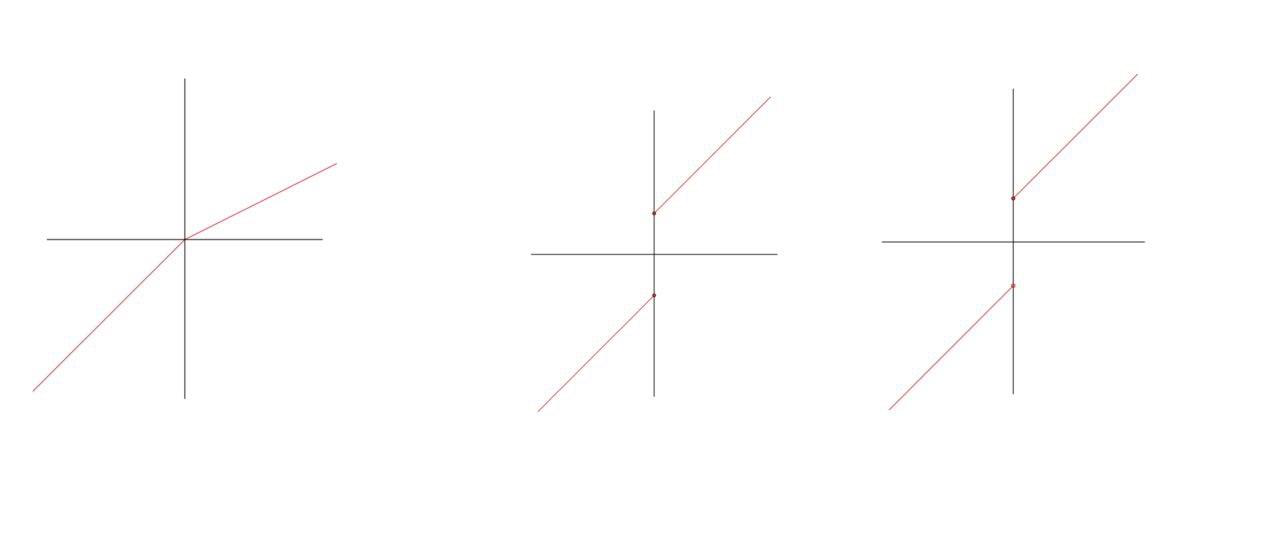
\includegraphics[scale = 0.2]{Figures/Chapter1/continuousFunctions.png}
                \caption{The mappings $h$, $k$, and  $l$.}
                \label{fig_1.9}
            \end{figure}
\end{example} 

\begin{theorem}\label{1.7.5}
    Let $f:A \rightarrow X \times Y$ be defined by  $f(a)=(f_1(a),f_2(a))$, where $ f_1:A
    \rightarrow X$ and $ f_2: A \rightarrow Y$. Then $f$ is continuous if and only if  $ f_1$ and $
    f_2$ are continuous.
\end{theorem}
\begin{proof}
    Let $\pi_1:X \times Y \rightarrow X$ and $\pi_2:X \times Y \rightarrow Y$ be projections onto
    $X$ and  $Y$ respectively. Since  $\pi_1^{-1}(U)=U \times Y$ and $\pi_2^{-1}(V)=X \times V$ are
    both open in  $X \times Y$,  $\pi_1$ and $\pi_2$ are continuous. Then notice that $ f_1(a)=\pi_1
    \circ f(a)$ and $ f_2(a)=\pi_2 \circ f(a)$, both of which are continuous.

    Now suppose that $ f_1$ and $ f_2$ are continuous..We have that $a \in f^{-1}(U \times V)$ if
    and only if $f_1(a) \in U$ and $ f_2(a) \in V$, then $ f_1^{-1}(U)$ and $f_2^{-1}(V)$ are open
    in $A$, hence so is $f^{-1}(U \times V)=f_1^{-1}(U) \cap f_2^{-1}(V)$.
\end{proof}

\begin{definition}
    We define the \textbf{parametrized curve} of the plane $\R^2$ to be the continuous function
    $f:[a,b] \rightarrow \R^2$ defined by $f(t)=(x(t),y(t))$. If $f$ is in a vector field, then wwe
    define $f(t)=x(t)i+y(t)j$ where $i=
    \begin{pmatrix}
        1 \\
        0
    \end{pmatrix}$
    and $j=
    \begin{pmatrix}
        0 \\
        1
    \end{pmatrix}$
\end{definition}

\begin{example}
    The function $f(t)=((\cos(t)),\sin(t))$ is a parametrization of the curve $x^2+y^2=1$, i.e. the
    unit circle  $S^1$.
\end{example} 
